This chapter provides detailed specifications of the system under development.

\section{Functional Requirements}
These functions are logically grouped into modules based on their purpose/users/mode of operations etc (as per our system). \\
\\
There are three primary actors involved in this system which includes the user, the admin and the system itself so we have broken down the functionality into three modules since each module has various functional components. \\
\\
The user modules includes all the functionality that is required by the user for the system to work that is clicking various buttons in order to get the system to work. The admin model includes the functionality required by the admin to get the app to work and lastly the system module to be functional in order for the app to be functional.  
\begin{outline}
  \1 \textbf{User Module}:
  \2 Function 1: User should be able to take capture an image by clicking the button.
  \2 Function 2: User should be able to log in and out of the system.
  \2 Function 3: User should be able to sign-up into the system.
  \2 Function 4: User should be able to add the job.
  \2 Function 5: User should be able to add some description while uploading the job.
  \2 Function 6: User should be able to view the jobs he has posted.
  \1 \textbf{Admin Module}:
  \2 Function 1: Admin should be able to log in and out of the system.
  \2 Function 2: Admin should be able to view the route.
  \2 Function 3: Admin should have all control of the system including the features on all of the portals.
  \2 Function 4: Admin should be able to view all the jobs that have been posted.
  \2 Function 5: Admin should be able to add and remove other admins.
  
  \1 \textbf{System Module}:
  \2 Function 1: System should be able to take a picture.
  \2 Function 2: System should be able to upload the job in the server.
  \2 Function 3: System should be able to pre-process the images which includes data cleaning.
  \2 Function 4: System should be able to identify garbage.
  \2 Function 5: System should be able to accept and reject images on the basis of identification.
  \2 Function 6: System should be able to quantify the garbage in the image.
  \2 Function 7: System should be able to generate a route.
  \2 Function 8: System should be able to display the generated route to the admin.
\end{outline}

% --- The above is to be modified as per your project, e.g. a flat list if your system has limited functional requirements.
\newpage
\section{Non-functional Requirements}

The primary non-functional requirements that lies in our system are:\\
\\
\textbf{Accessibility}:
Accessibility is regarded as the ability to access or benefit from the system. The application will be directly/indirectly accessed and compatible with latest technology by a wide range of people. Whenever the application is accessed on any user device it should be operate-able.\\
\\
\textbf{Availability}: 
Availability is regarded as the total time an application is capable of being used during a time period. The application will be available and operate-able throughout the day with down time percent $<0.9998$.\\
\\
\textbf{Durability}: 
Durability is regarded as the application being functional without requiring any excessive maintenance and repair. The application will remain functional, without requiring excessive maintenance or repair, when faced with challenges of normal operation.\\
\\
\textbf{Integrability}: 
The application will be able to bring all sub-systems together in one single system and is able to deliver its functionality. The system will be able to coordinate will all its sub system which includes the machine learning model, database and the cloud server.\\
\\
\textbf{Maintainability}:
Maintainability is regarded as the continuous improvements of the system. The system developed should be easy to maintain. In case of any errors, it should be easy for the maintenance team to repair that error with utilizing minimum resources.\\
\\
\textbf{Reliability}:
Reliability is said to be that the system is able to function under stated conditions and for a specified period of time. Hence the system will be reliable while performing any task, it should not fail while performing the same task again. The failure ratio should be minimized.



\newpage
\section{External Interfaces}

\subsection{User Interfaces}
The Mockups are divided into two categories:\\
1- The User Panel (Mobile Application) \\
2- The Admin Panel (Web Application)\\
\\
\textbf{User Panel:}
The User Panel will provide the user with two options. They can choose to either sign in to the system using and ID and password which they previously created or sign up into the system if they are using the application for the first time. 


\begin{figure}[!hb]
   \centering
   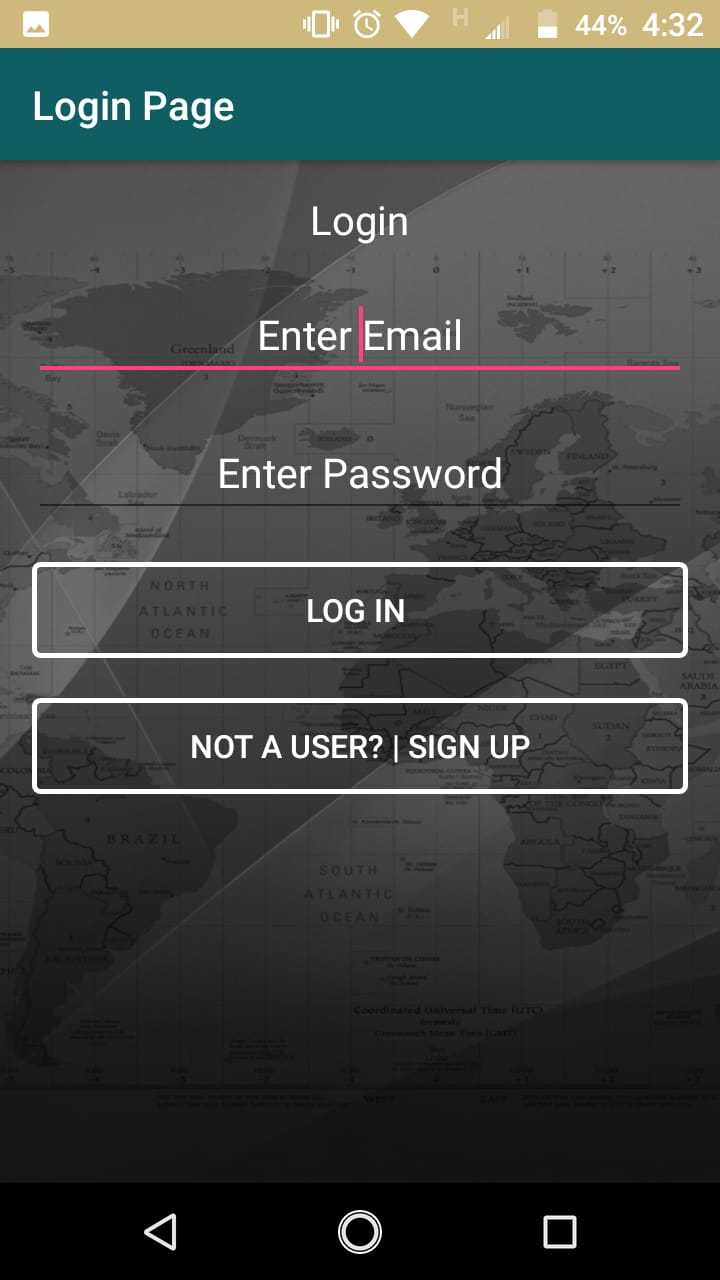
\includegraphics[scale=0.5]{images/1.png}
   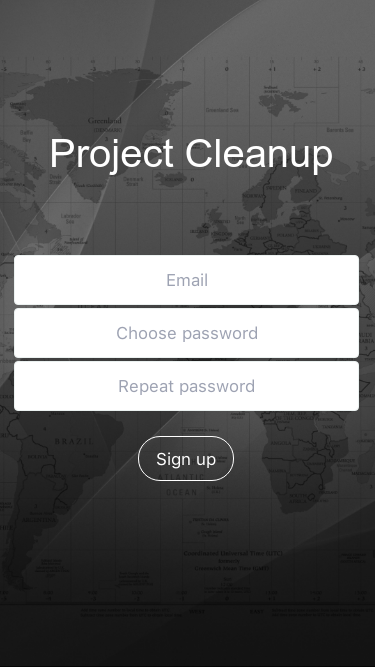
\includegraphics[scale=0.5]{images/2.png}

 
   \caption{User Panel}\label{fig:picture}
\end{figure}
\newpage
\begin{figure}[!hb]
   \centering

   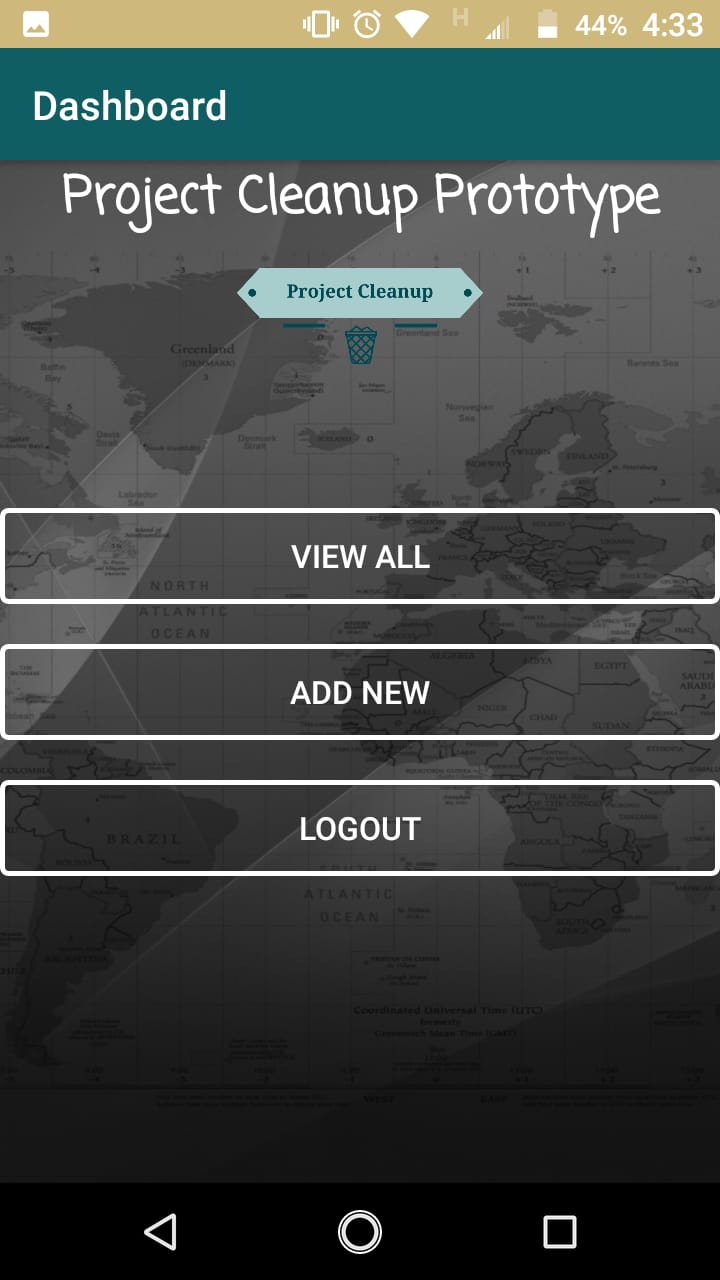
\includegraphics[scale=0.5]{images/3.png}
   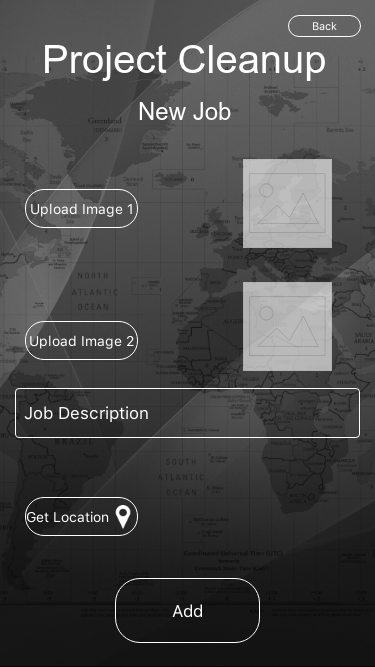
\includegraphics[scale=0.5]{images/4.png}
   
 
   \caption{User Panel}\label{fig:picture}
\end{figure}
After logging in, the user is presented with two options. A user can either add a new job or view the job list that is his/her previously submitted requests.\\
If the user clicks on add new job the app displays a new screen which asks the user to upload two images. User can also using the description box to add comments if he wants to. The user is then supposed to add the job which is a process of submitting his request. It is important to note that the location must be turned on in order to add the job.\\
The screens also consist of the "back" option.
If the User chooses the view jobs option and clicks on it then a new screen appears which shows the job list, that is previously submitted requests. This screen also consists of a back button.\\
\newpage
\begin{figure}[!hb]
   \centering

   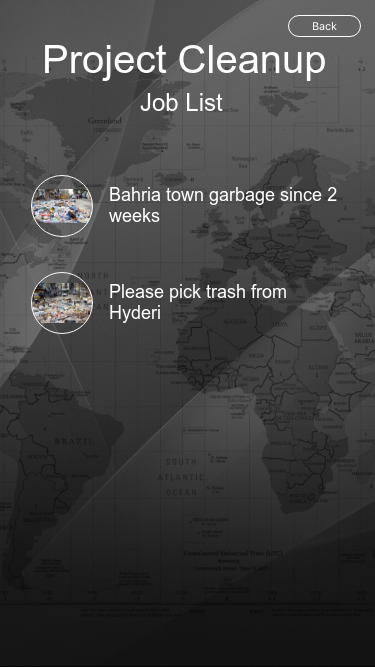
\includegraphics[scale=0.5]{images/5.png}
 
   
 
   \caption{User Panel}\label{fig:picture}
\end{figure}

\textbf{Admin Panel:}
The admin panel will be available on the web application. The web application will consist of an admin login screen. Through that screen the admin will be able to put in the ID and Password that he is assigned which will be authenticated and once that is done the admin will be able to log in.\\
\\
The admin will be able to do two tasks:\\
1)Admin will be able to view all the job requests that were submitted by the users.\\
2)The admin will also be able to view the route on the admin panel.

\newpage
\begin{figure}[!hb]
   \centering

   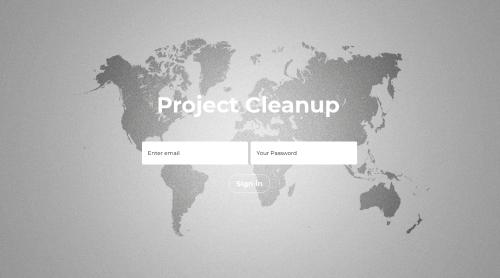
\includegraphics[scale=0.8]{images/6.png}
 \\
   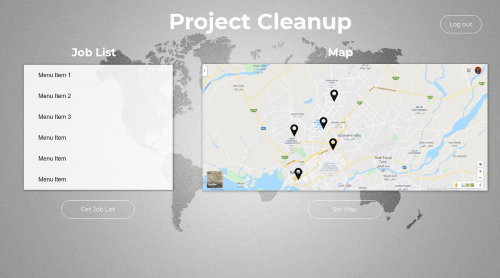
\includegraphics[scale=0.8]{images/7.png}
 
   \caption{Admin Panel}\label{fig:picture}
\end{figure}
\subsection{Application Program Interface (API)}
Our complete model will be able to take an image as input, identify segments of garbage and approximately quantify the volume of garbage,. Once our model has been made and is able to process data according to our requirements We will be uploading this model to a cloud server. AWS Lambda is one of the leading platforms for hosting models on cloud servers. 

In order for any client to use the model on the server we need a communication protocol. Once our model is on the cloud, AWS Lambda provides us with an application programming interface that can be easily connected with any interface of an application to use.
\newpage
\subsection{Hardware/Communication Interfaces}
This section describes the tools and technologies will be using for the different components of our project.\\
\textbf{Phone Application}:\\
For the user interface that is the front end we will be using ionic which is focused mainly on the look and feel and we think it will work best fro the UI interaction and the framework we would be using is React native. Our application will be for android users.\\
\textbf{Web Application}:\\
For the Web Application we will be using Javascript MVC Frameworks Angular JS/django node both of which are open source tools known for writing quick to write and powerful client-side web applications. We will also be using React, a javascript library, to make an interactive experience for the user.\\
\textbf{Cloud Server:}\\
We will be using AWS lambda as the cloud server AWS Lambda is one of the leading platforms for hosting models on cloud servers.AWS Lambda provides us with an application programming interface that can be easily connected with any interface of an application to use.\\
\textbf{Database:} \\
We will be exploring AWS and Firebase Database and use what works best for us.While we will be using MySQL which is a relational database management system based on SQL – Structured Query Language as backup.
\begin{figure}[!hb]
   \centering

   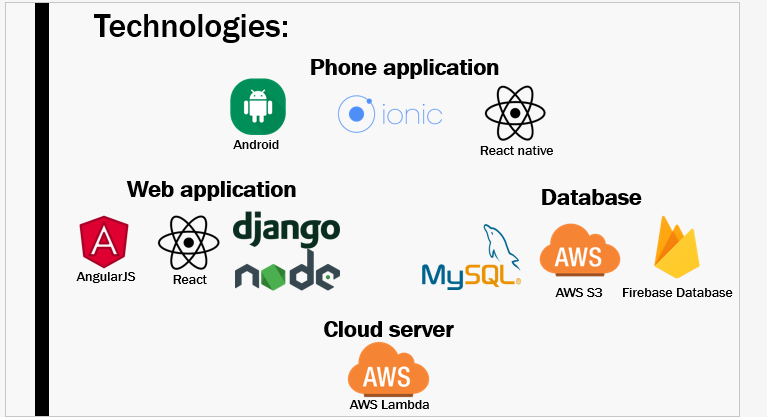
\includegraphics[scale=0.5]{images/Tech.PNG}

 
   \caption{Tools and Technologies}\label{fig:picture}
\end{figure}
\newpage
\section{Use Cases}
This section presents detailed use cases of our system.
\subsection{Admin:}
\begin{figure}[!hb]
   \centering

   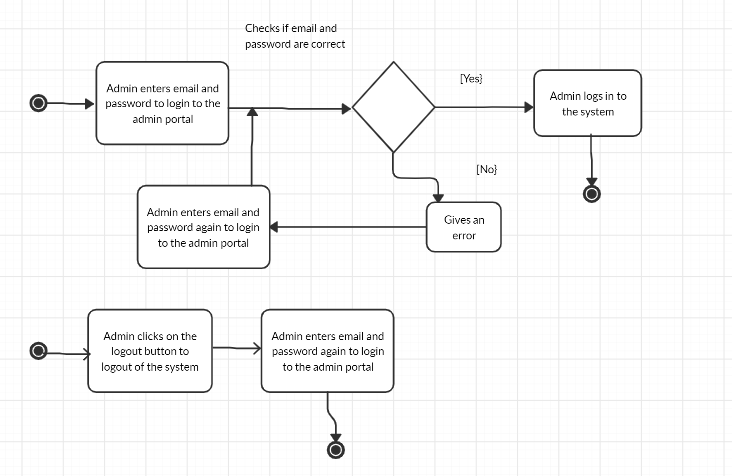
\includegraphics[scale=0.6]{images/Admin_1.PNG}

 

\end{figure}

\begin{figure}[!hb]
   \centering

   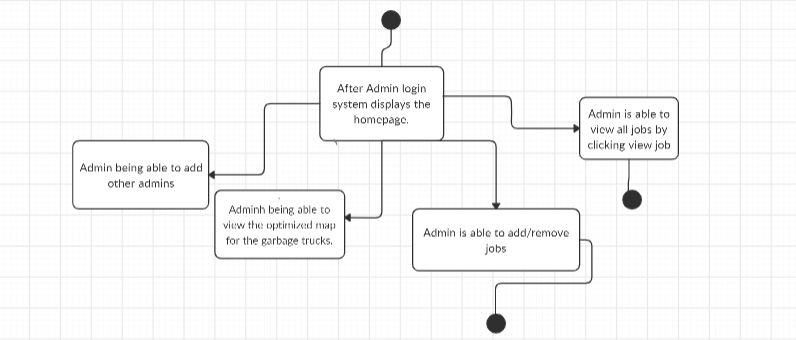
\includegraphics[scale=0.6]{images/Admin_3.PNG}
\end{figure}
\newpage
\subsection{User:}
\begin{figure}[!hb]
   \centering

   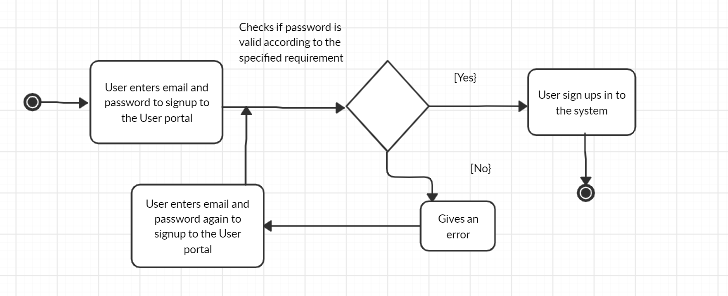
\includegraphics[scale=0.4]{images/User.PNG}
\end{figure}
\begin{figure}[!hb]
   \centering

   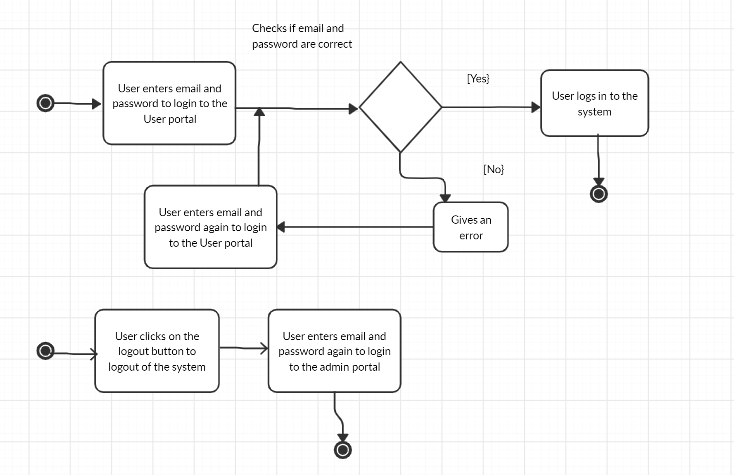
\includegraphics[scale=0.4]{images/User_1.PNG}
\end{figure}
\begin{figure}[!hb]
   \centering

   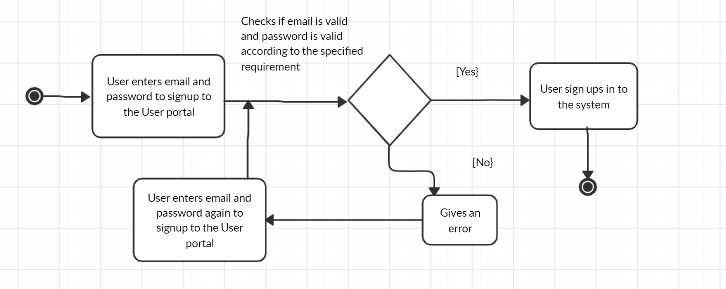
\includegraphics[scale=0.4]{images/User_2.PNG}
\end{figure}
\begin{figure}[!hb]
   \centering

   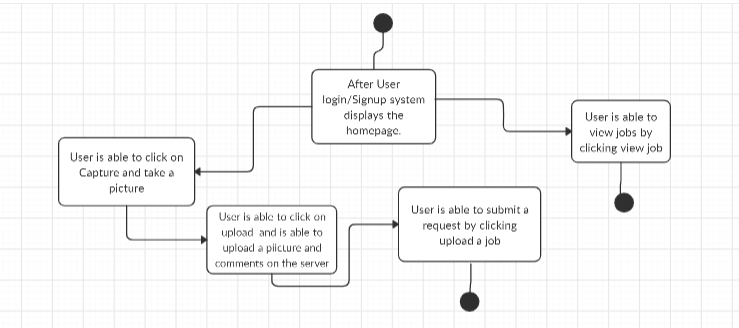
\includegraphics[scale=0.4]{images/User_3.PNG}
\end{figure}
\newpage
\subsection{System:}
The system activity diagram is divided into two parts: \\
The flow of the process and the decision making involved in the process. The flow of the process is from  the perspective of the user and the procedure explains the entire process happening behind the scenario that is after the user submits a request, the working of the system.

\begin{figure}[!hb]
   \centering

   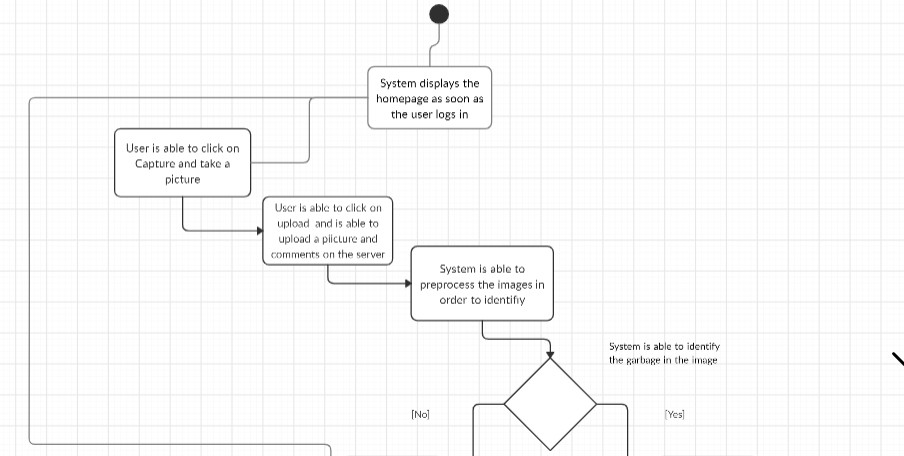
\includegraphics[scale=0.6]{images/UserSystem_1.PNG}
   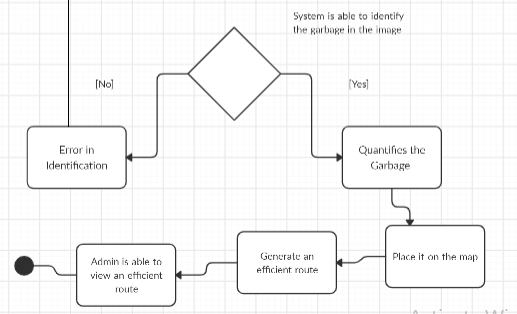
\includegraphics[scale=0.6]{images/UserSystem_2.PNG}
   
\end{figure}

\newpage
\section{Datasets}
One of the most important component of our project is the identification of the garbage and after our primary research we found out that work has been done on it and so we will be testing that out to incorporate it in our project. The application that works on the identification is called SpotGarbage.\\
We will be using their dataset which can be found at:\\
Garbage In Images (GINI) Dataset (https://github.com/spotgarbage/spotgarbage-GINI)\\
The dataset consists of categories of garbage and non-garbage, queries and non-queried images and  ambiguous annotated images. \\
\\
These categories further consist of garbage at various locations, litter, railway garbage, waste, street garbage, kitchen waste while non garbage images include buildings, chaos, streets, city, crowd, nature, texture, fruits and vegetables, earth+dust etc.\\
\\
We will also be creating our own dataset taking pictures of garbage from two different angles for the quantification component.

\begin{figure}[!hb]
   \centering

   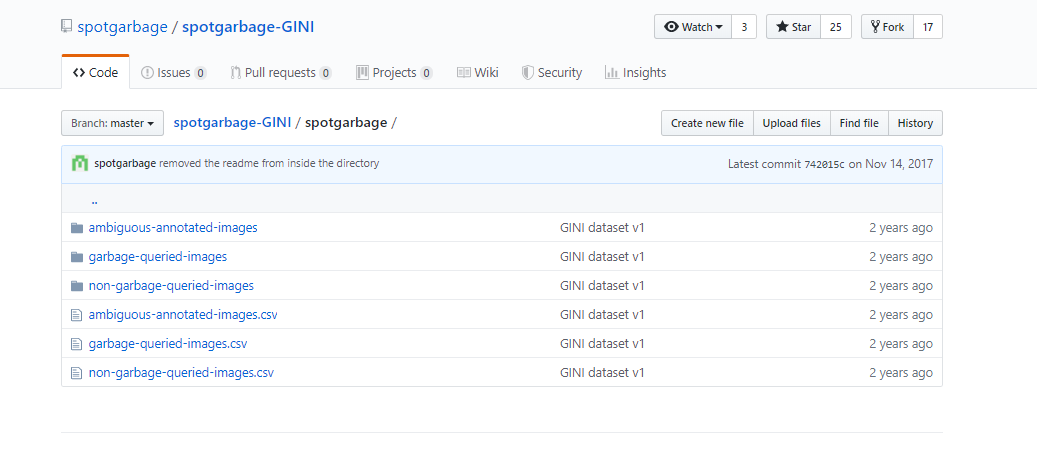
\includegraphics[scale=0.7]{images/Dataset.PNG}

 
   \caption{Dataset}\label{fig:picture}
\end{figure}
\newpage
\section{System Diagram}
This diagram gives a high-level view of the different components of our system and the interactions between them.\\
\textbf{User  app:}\\
Front end: ionic / Android / react native\\
Back end: Firebase Database\\
(Described in section 3.3.3)\\
\\
\textbf{Admin panel:}\\
Front end: Angular/ React\\
Back end: NodeJS / Django with Firebase Database\\
(Described in section 3.3.3)\\
\\
\textbf{Model Preprocessing:}\\
Python-OpenCV library:OpenCV is a Python library which is designed to solve computer vision problems.
\\
\textbf{Spotgarbage}:\\
Python-Caffe library:Caffe is good for fast training and testing, so if you want to experiment on different neural net architectures then it's a great choice because you don't even need to write code to design a neural net and things like fine tuning/transfer learning is extremely easy.\\
\\
Open-CV
\\
Pil:The Python Imaging Library (PIL) adds image processing capabilities to your Python interpreter.\\
\\
Numpy:Numpy is a general-purpose array-processing package. It provides a high-performance multidimensional array object, and tools for working with these arrays. It is the fundamental package for scientific computing with Python.\\
\\
\textbf{Quantification}: \\
Python image processing libraries\\
\\
\textbf{Cloud}:\\
AWS Lambda dependencies
\newpage
\textbf{System Diagram:}\\
\\
The system diagram is as follows:
\begin{figure}[!hb]
   \centering
   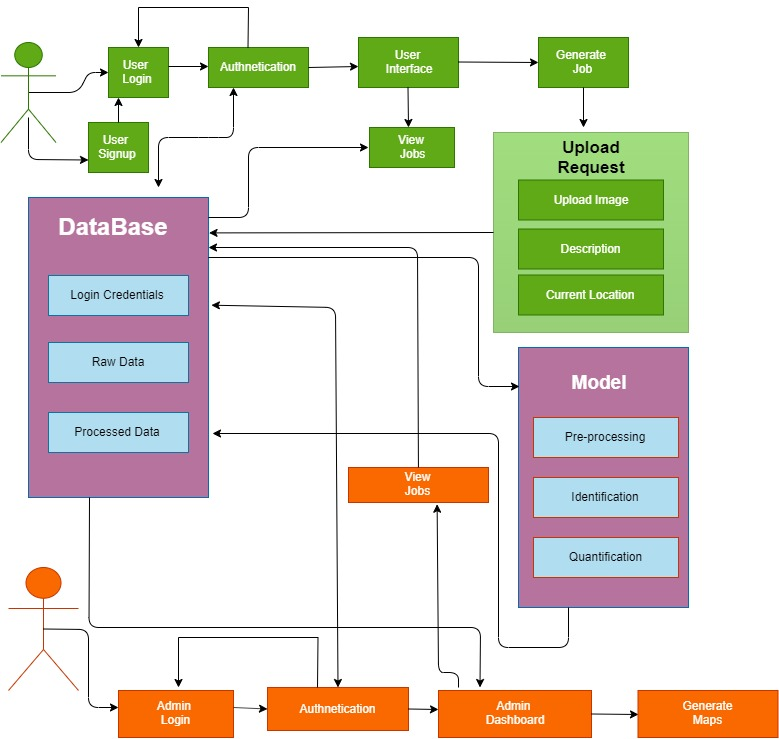
\includegraphics[scale=0.5]{images/8.jpeg}
   \caption{A Picture}\label{fig:picture}
\end{figure}